\documentclass[conference, a4paper]{IEEEtran}
\IEEEoverridecommandlockouts
\usepackage{cite}
\usepackage{url}
\usepackage{amsmath,amssymb,amsfonts}
\usepackage{algorithmic}
\usepackage{graphicx}
\usepackage{textcomp}
\usepackage{xcolor}
\usepackage{booktabs}
\usepackage{tabularx}
\usepackage{multirow}

\usepackage{tikz}
\usetikzlibrary{shapes.geometric, arrows, positioning, fit, backgrounds}

\def\BibTeX{{\rm B\kern-.05em{\sc i\kern-.025em b}\kern-.08em
    T\kern-.1667em\lower.7ex\hbox{E}\kern-.125emX}}

\begin{document}

\title{Multi-Environment TinyML Calibration of a Low-Cost Pan-Tilt Time-of-Flight LiDAR for Indoor 3D Reconstruction}

\author{\IEEEauthorblockN{Anonymous Authors}
\IEEEauthorblockA{\textit{Affiliations removed for double-blind review}}
}

\maketitle

\begin{abstract}
Single-point time-of-flight (ToF) sensors provide a low-cost alternative to mechanically scanned LiDAR for indoor mapping, but their ranging accuracy is sensitive to target reflectivity, ambient illumination, multipath interference, and scan geometry. This paper presents a low-cost pan-tilt ranging platform built around a VL53L1X ToF sensor and an ESP32 microcontroller, and evaluates machine-learning-based residual calibration across two substantially different indoor acquisition campaigns. The first campaign was conducted in a relatively controlled, low-ambient-light room, whereas the second introduced stronger LED illumination, painted concrete surfaces, cardboard obstacles, and translucent objects. Cross-environment transfer experiments show that a model trained in one environment does not reliably transfer to the other: XGBoost produced mean absolute errors (MAEs) of 947.15 mm when trained on the controlled environment and tested on the diverse environment, and 1049.09 mm in the reverse direction. In contrast, pooled training across both environments reduced the combined-dataset MAE from 149.84 mm for the uncalibrated sensor to 22.41 mm with XGBoost. For embedded deployment, a single decision tree with maximum depth 12 achieved 23.42 mm test MAE, required 453.8 KB of generated C source code, and executed in under 100 microseconds on the ESP32, which is negligible relative to the sensor's 50 ms timing budget. These results demonstrate the practical value of multi-environment calibration for low-cost ToF mapping while also showing that environment-specific models can fail severely outside their training domain. Because the present pooled evaluation uses only the two observed environments, performance on a completely unseen environment remains an open question.
\end{abstract}

\begin{IEEEkeywords}
Time-of-Flight, LiDAR, sensor calibration, TinyML, edge AI, ESP32, indoor mapping, point cloud.
\end{IEEEkeywords}

\section{Introduction}
Indoor 3D mapping is crucial for mobile robotics, structural inspection, and augmented reality \cite{hess2016real, rusu20113d}. Commercial LiDAR systems can provide high accuracy and dense measurements, but their cost and power requirements may be unsuitable for educational platforms, low-cost robotics, and embedded sensing applications \cite{amann2001laser, behroozpour2017lidar}. A common low-cost alternative is to mount a single-point ToF sensor on a two-axis pan-tilt mechanism and convert sequential range measurements into a 3D point cloud \cite{willis2009design}.

The practical limitation of this approach is measurement reliability. Low-cost ToF sensors are affected by multipath interference (MPI), target reflectivity, ambient infrared radiation, and angular scanning geometry \cite{corti2016metrological, lindner2010time}. In mechanically actuated platforms, these optical effects are further coupled with servo non-linearity and alignment error. Consequently, a calibration model that performs well in one room may not remain accurate when lighting, wall material, or scene geometry changes.

Machine learning practically models nonlinear residual errors without exhaustive analytical derivation \cite{he2017depth}. However, two issues remain: the calibration model should be evaluated across different acquisition conditions, and the final model must fit a microcontroller.

This work addresses these issues using a VL53L1X-based pan-tilt scanner. Alongside measured distance and commanded angles, we record sensor telemetry (signal and ambient return rates) to capture measurement context. We then compare environment-specific calibration with pooled multi-environment calibration and study the accuracy-memory trade-off required for ESP32 deployment.

The main contributions of this paper are as follows:

\begin{enumerate}
\item \textbf{Cross-environment transfer analysis:} We quantify the failure of an ML calibration model when it is trained in one acquisition environment and evaluated in another with substantially different lighting, materials, and scene conditions.
\item \textbf{Multi-environment pooled calibration:} We show that combining data from both observed environments enables substantially lower overall calibration error than either the raw sensor or single-environment transfer models.
\item \textbf{Embedded TinyML deployment:} We identify a compact decision-tree model that retains most of the accuracy of the higher-capacity model while fitting the memory and latency constraints of the ESP32.
\end{enumerate}

Importantly, the pooled evaluation in this study should be interpreted as multi-environment calibration over the two observed domains rather than strict unseen-domain generalization. Evaluation on an independent third environment is left for future work.

\section{Related Work}

\subsection{ToF Sensor Error Characterization}
The error characteristics of time-of-flight sensors are strongly influenced by optical and geometric conditions. Dark or weakly reflective targets reduce returned photons and increase measurement uncertainty, while strong ambient illumination degrades the signal-to-background ratio \cite{corti2016metrological, foix2011lock, hansard2012time}. Measurement error varies with target distance, device temperature, and material properties \cite{frangez2022assessment, kahlmann2006calibration, wasenmuller2016comparison}. Multipath interference (MPI) introduces bias when emitted light reaches the receiver along more than one optical path, as occurs near corners, reflective surfaces, or translucent objects \cite{sabov2008identification, reynolds2011capturing, dorrington2011separating}. Early calibration work on the SwissRanger demonstrated that systematic ToF errors can be modeled and corrected through device-specific calibration tables \cite{kahlmann2006calibration, fuchs2008extrinsic}, while lateral and depth calibration of PMD sensors established foundational methods for combined geometric-radiometric correction \cite{lindner2006lateral}. These approaches, however, require per-device analytical models that may not generalize across operating conditions.

\subsection{Machine Learning for Depth Correction}
Data-driven depth correction offers an alternative to analytical calibration. DeepToF demonstrated that learned models map complex ToF distortions to corrected depth \cite{su2018deeptof}. Convolutional models further reduce MPI artifacts by exploiting spatial context \cite{agresti2018deep}, with ongoing research exploring learning-based MPI correction \cite{guo2021tackling}. He et al. formalized residual error analysis for ToF cameras using signal-dependent correction models \cite{he2017depth}, while Mersmann et al. applied ToF calibration to intraoperative surface reconstruction \cite{mersmann2013calibration}. Jung et al. addressed joint calibration of color-depth camera pairs \cite{jung2015tof}. Most high-capacity approaches target imaging cameras or GPU-capable systems. In contrast, this work addresses a single-point ToF sensor on a low-cost scanner, emphasizing cross-environment robustness and microcontroller deployment.

\subsection{Low-Cost LiDAR and Indoor Mapping}
Low-cost 3D scanning has been achieved by mechanically rotating single-point or 2D LiDAR sensors \cite{willis2009design, fpga2019lowcost, low2024cost3d, jimenez20143d, kim2015design}, sharing the challenge of calibrating errors from mechanical scanning and varying conditions.

\subsection{TinyML and Edge-Based Calibration}
TinyML focuses on executing learned models on resource-constrained embedded devices \cite{hayajneh2024tinyml, wang2020tinyml, warden2019tinyml, lin2020mcunet}. Benchmarking efforts have standardized TinyML evaluation \cite{banbury2021benchmarking}, while TensorFlow Lite Micro enables neural network deployment on microcontrollers \cite{david2021tensorflow}. For tree-based models, inference reduces to conditional branches with minimal dependencies. Tools such as \texttt{m2cgen} transpile trained scikit-learn \cite{pedregosa2011scikit} estimators into C code for direct sensor-loop integration.

\section{Methodology}

\subsection{Hardware Platform}
The sensing device consists of a VL53L1X single-point ToF module \cite{stmicro2018vl53l1x} mounted on a custom 3D-printed pan-tilt assembly actuated by two SG90 micro-servos. An ESP32-WROOM-32 development module \cite{espressif2023esp32} controls the servos and communicates with the ToF sensor over I2C at 400 kHz. A DHT11 temperature sensor and an INA219 power-monitoring module record environmental and system variables. The servos were isolated and powered by an independent Arduino Nano to provide a stable 5V supply and prevent ESP32 brownouts during actuation. The VL53L1X timing budget was configured to 50 ms per ranging cycle.


The servo exhibits non-uniform angular error. Rather than applying mechanical correction tables, commanded angles are included directly in the feature vector, allowing the model to learn angle-dependent residuals automatically.

\begin{figure}[htbp]
\centering
\begin{minipage}{0.48\columnwidth}
  \centering
  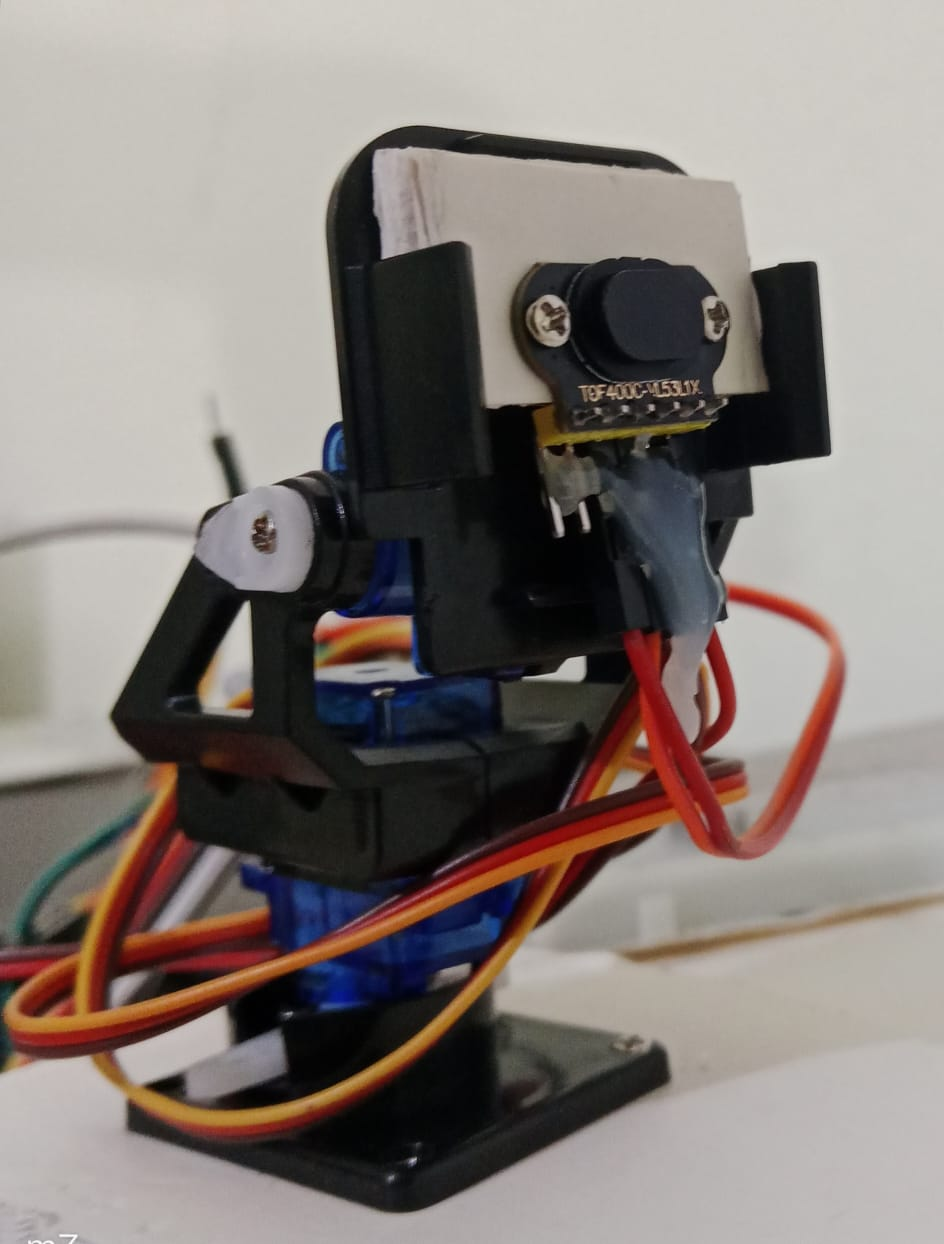
\includegraphics[width=\linewidth]{figures/TOF 400cVL53L1X sensor attached with 2 sg-90 servo.png}
  \caption{Assembled pan-tilt rig wired to ESP32.}
  \label{fig:sensor_setup}
\end{minipage}\hfill
\begin{minipage}{0.48\columnwidth}
  \centering
  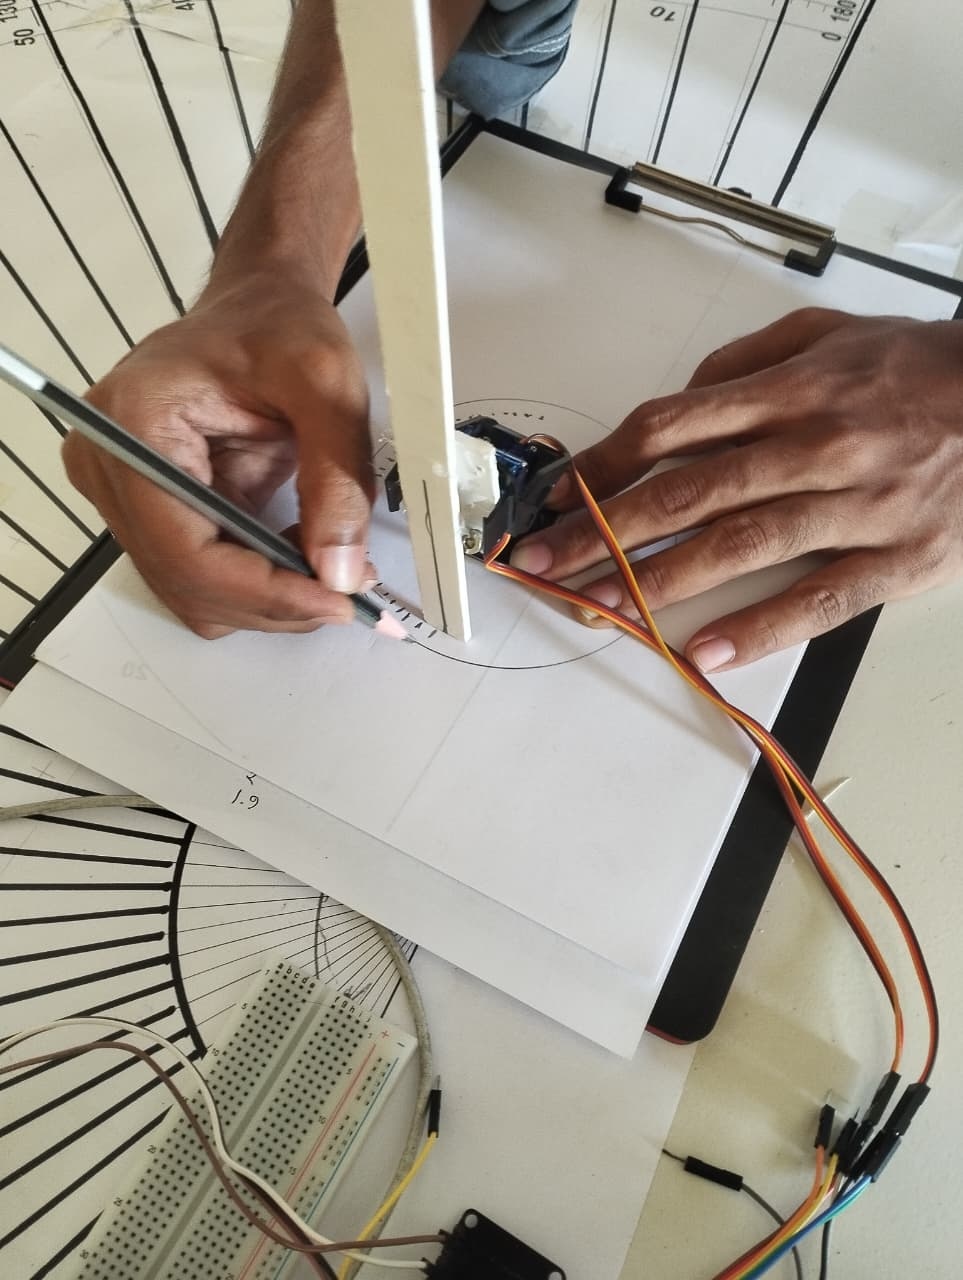
\includegraphics[width=\linewidth]{figures/servo_angles.jpeg}
  \caption{Rig actively measuring servo angles.}
  \label{fig:hardware}
\end{minipage}
\end{figure}

\subsection{Data Collection}
Data were collected in two campaigns on separate days in different indoor spaces to expose the sensor to different lighting, surface, and scene conditions (Table~\ref{tab:dataset}).

\begin{table}[htbp]
\centering
\caption{Dataset Characteristics and Acquisition Conditions}
\label{tab:dataset}
\begin{tabular}{@{}lcc@{}}
\toprule
\textbf{Metric} & \textbf{Day 1 (Controlled A)} & \textbf{Day 2 (Diverse B)} \\ \midrule
Environment & Dark room, uniform walls & Hallway, LED lit, boxes \\
Trainable Rows & 51,000 & 8,477 \\
Total Valid Returns & 53,539 & 9,104 \\
Pan Range & $0^\circ$ to $180^\circ$ & $20^\circ$ to $160^\circ$ \\
Tilt Range (Raw) & $0^\circ$ to $179.9^\circ$ & $70^\circ$ to $150^\circ$ \\
Lighting & Low/controlled ambient & Extreme variations \\
\bottomrule
\end{tabular}
\end{table}

In Environment A, a large reference was generated using a custom tiled protractor. Angular lines were extended toward the walls, and radial ground-truth distances were measured manually using a laser tape measure ($\pm$1 mm resolution) with an estimated $\pm$1$^\circ$ manual alignment uncertainty. Over 53,000 valid measurements were collected before filtering.

\begin{figure}[htbp]
\centerline{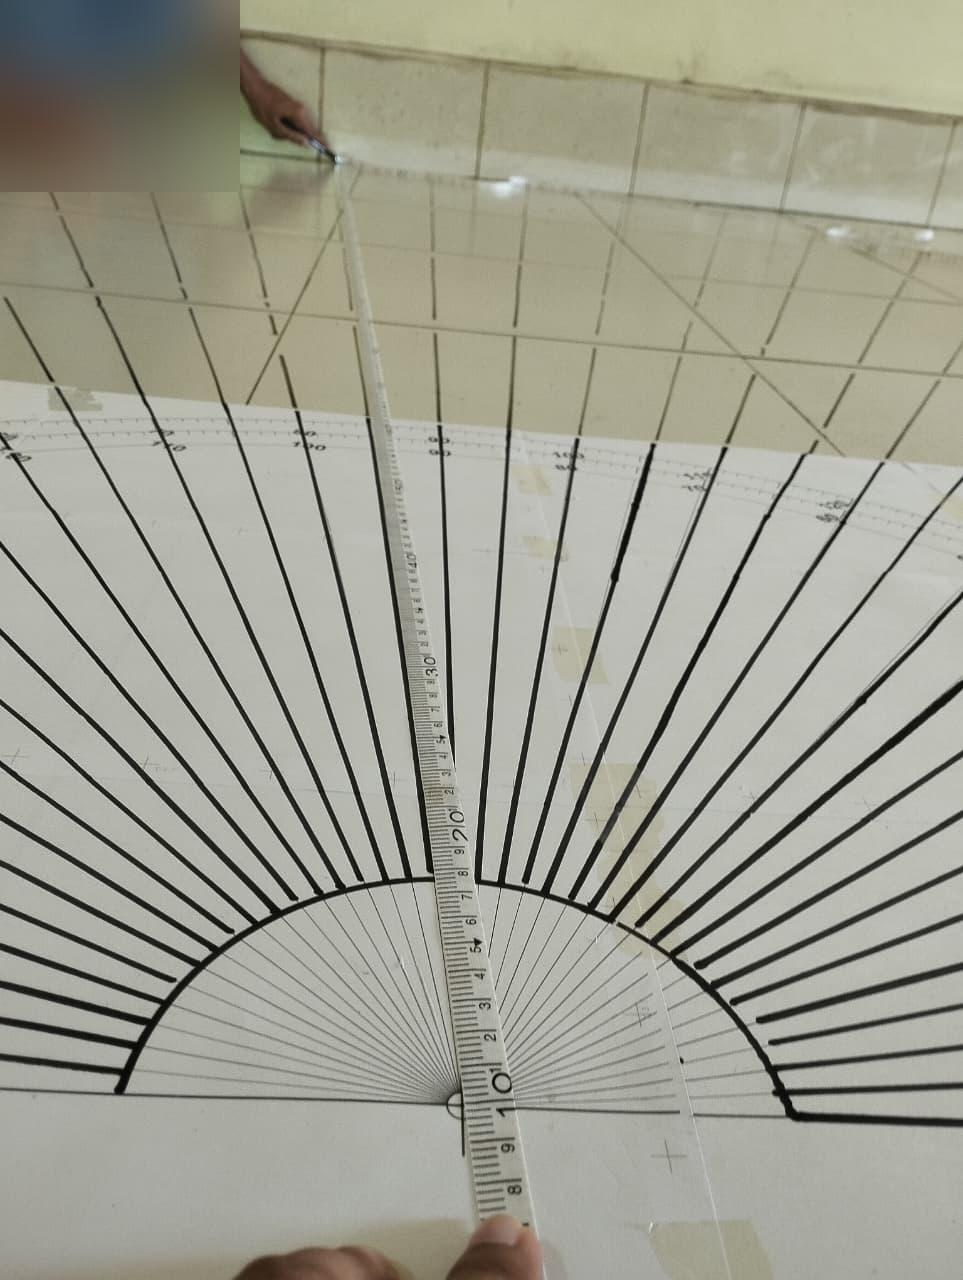
\includegraphics[width=0.7\columnwidth]{figures/measuring_ground_truth_blurred.jpeg}}
\caption{Ground-truth setup during Day 1. A custom-printed tiled protractor defines angular reference lines on the floor, while a precise measuring tool maps the true distance to the walls.}
\label{fig:groundtruth}
\end{figure}

Environment B introduced a wider range of conditions. Ten scans were recorded under varying LED illumination (partial, full, dark). Cardboard, translucent plastic, highly reflective white, and absorptive dark surfaces were introduced to trigger complex reflectance and multipath errors. Of 11,337 raw measurements, 9,104 valid sensor returns were recorded, and 8,477 were retained as trainable rows after excluding 627 samples due to out-of-bounds sensor timeouts or feature extraction failures.

\begin{figure}[htbp]
\centering
\begin{minipage}{0.48\columnwidth}
  \centering
  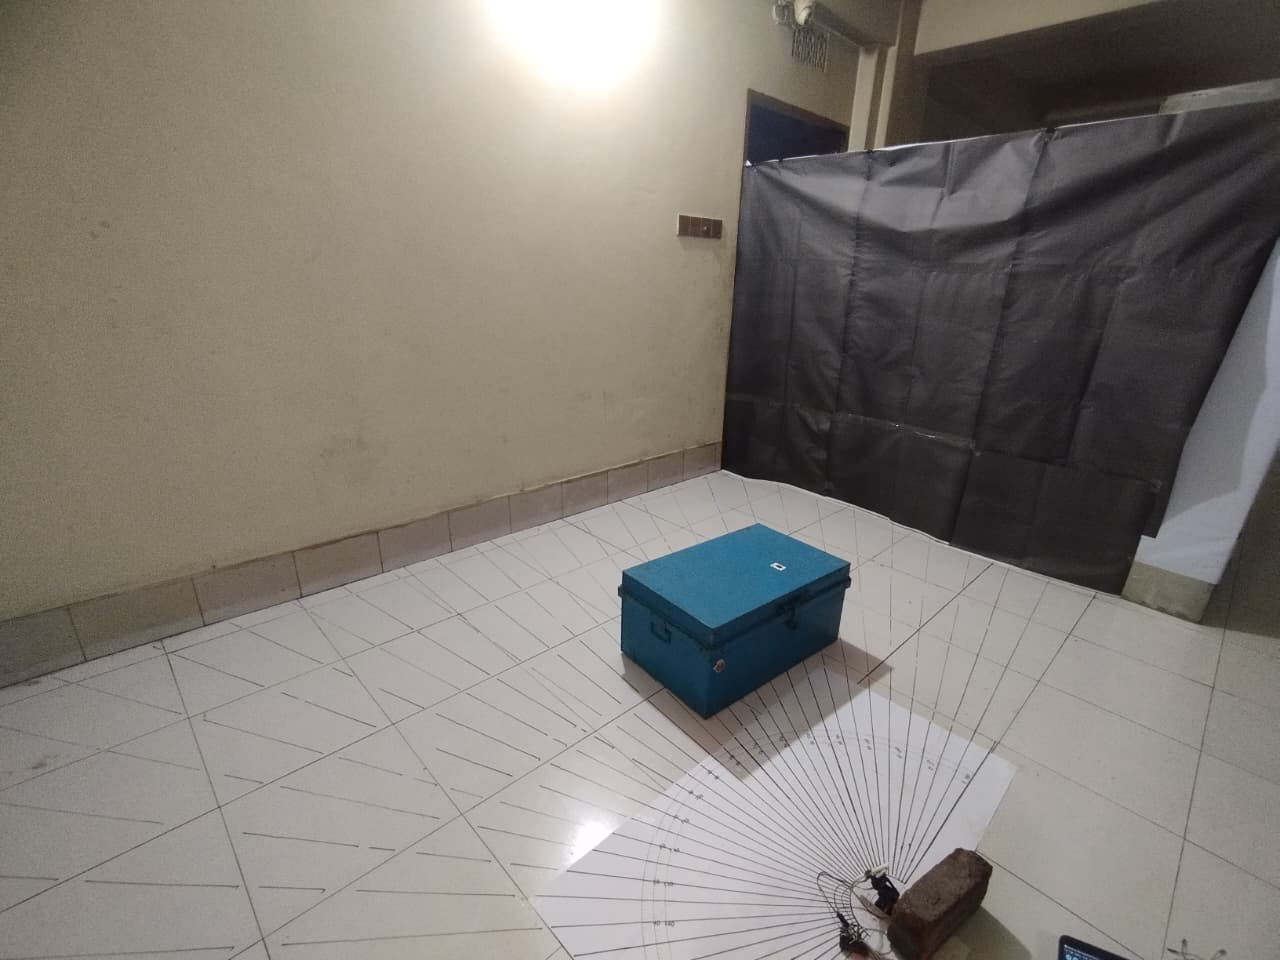
\includegraphics[width=\linewidth]{figures/day2_box.jpeg}
  \centerline{(a) Box with low-reflectivity wall}
\end{minipage}\hfill
\begin{minipage}{0.48\columnwidth}
  \centering
  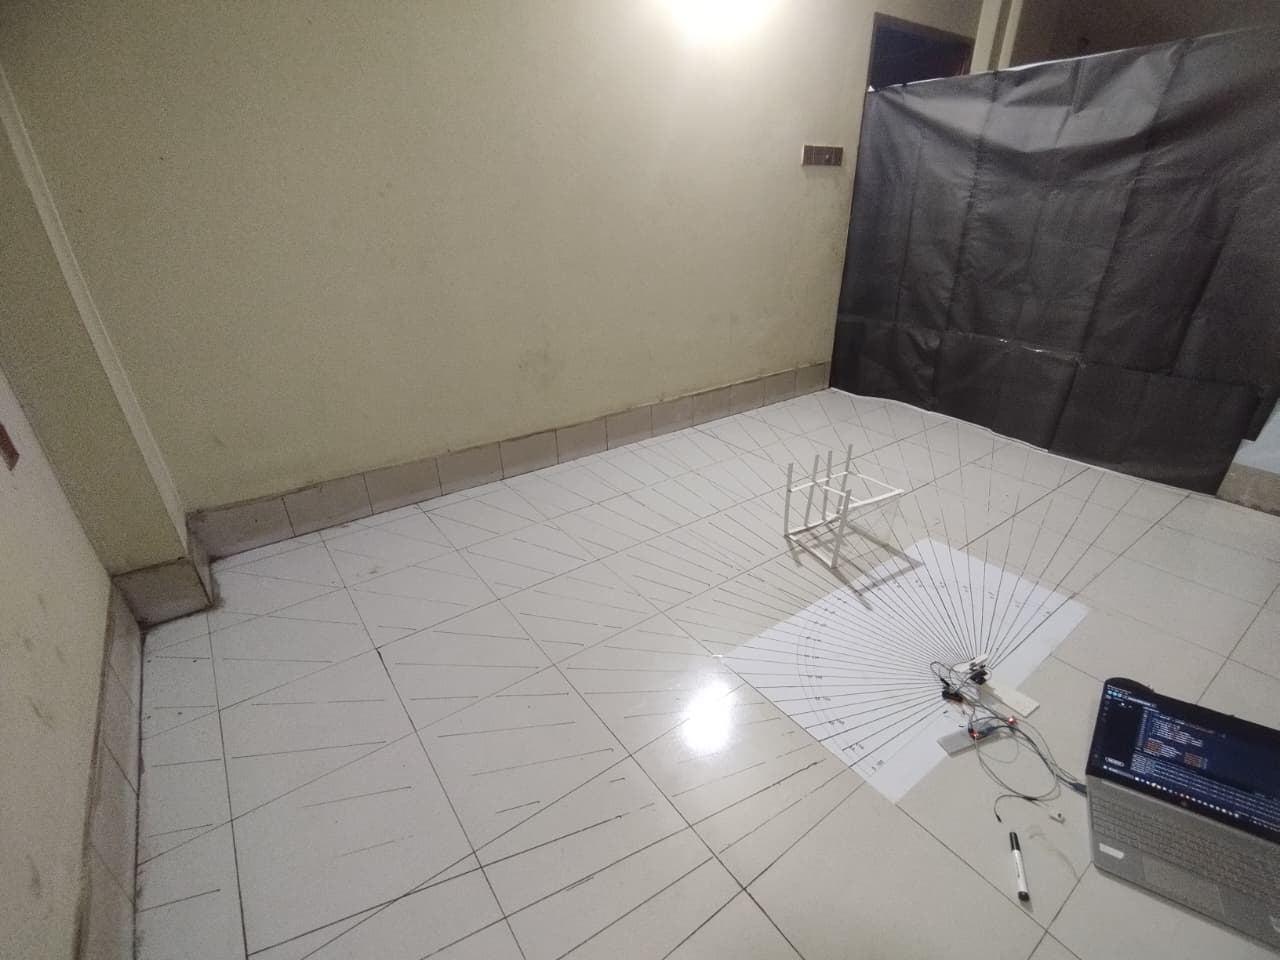
\includegraphics[width=\linewidth]{figures/day2_transparent.jpeg}
  \centerline{(b) Translucent object in path}
\end{minipage}
\caption{Physical setup of the Environment B (Day 2) testbed. The complex scenarios feature varied lighting conditions, low reflectivity surfaces, and translucent obstacles designed to aggressively challenge the raw sensor.}
\label{fig:day2_setup}
\end{figure}

\subsection{Residual Calibration Formulation}
Following the residual error modeling approach established in prior ToF calibration literature \cite{he2017depth, lindner2010time}, the learning problem is formulated as residual correction rather than absolute range prediction. Let $r_{raw}$ denote the measured ToF range and $r_{GT}$ the corresponding geometric ground truth. The residual target is:
\begin{equation}
e = r_{GT} - r_{raw}
\end{equation}
The model predicts $\hat e$, and the corrected distance is computed as:
\begin{equation}
r_{corr} = r_{raw} + \hat e
\end{equation}
The feature vector contains measured range, commanded pan angle $\theta$, tilt angle $\phi$, signal return rate, ambient return rate, and ambient temperature.

\begin{figure}[htbp]
\centering
\resizebox{\columnwidth}{!}{
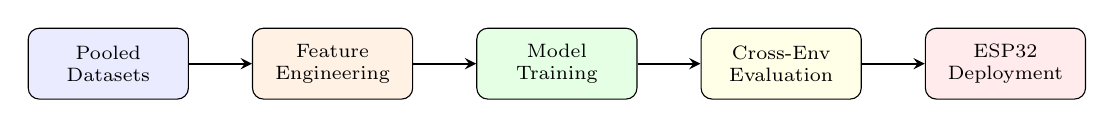
\begin{tikzpicture}[
    node distance=0.6cm and 0.8cm,
    block/.style={rectangle, draw, fill=blue!8, text width=1.8cm, text centered, rounded corners, minimum height=0.9cm, font=\scriptsize},
    arrow/.style={thick,->,>=stealth}
]
% Row 1: Data Collection
\node [block] (data) {Pooled\\Datasets};
\node [block, right=of data, fill=orange!10] (feat) {Feature\\Engineering};
\node [block, right=of feat, fill=green!10] (train) {Model\\Training};
\node [block, right=of train, fill=yellow!10] (eval) {Cross-Env\\Evaluation};
\node [block, right=of eval, fill=red!8] (deploy) {ESP32\\Deployment};

\draw [arrow] (data) -- (feat);
\draw [arrow] (feat) -- (train);
\draw [arrow] (train) -- (eval);
\draw [arrow] (eval) -- (deploy);
\end{tikzpicture}
}
\vspace{0.1cm}
\caption{Experimental workflow: data from two environments are pooled, features extracted, models trained (XGBoost \cite{chen2016xgboost}, Random Forest \cite{breiman2001random}, Decision Tree), evaluated across environments, and the optimal tree deployed on-device.}
\label{fig:workflow}
\end{figure}

\subsection{Evaluation Protocol}
Three evaluation settings are considered: (1) XGBoost trained on Environment A and tested on B, (2) training/test reversed, and (3) pooled training and evaluation on the combined dataset. For embedded experiments, an 80/20 train/test split evaluates models on unseen data. The primary metric is mean absolute error (MAE) in millimeters.

\section{Experimental Results}

\begin{figure*}[htbp]
\centerline{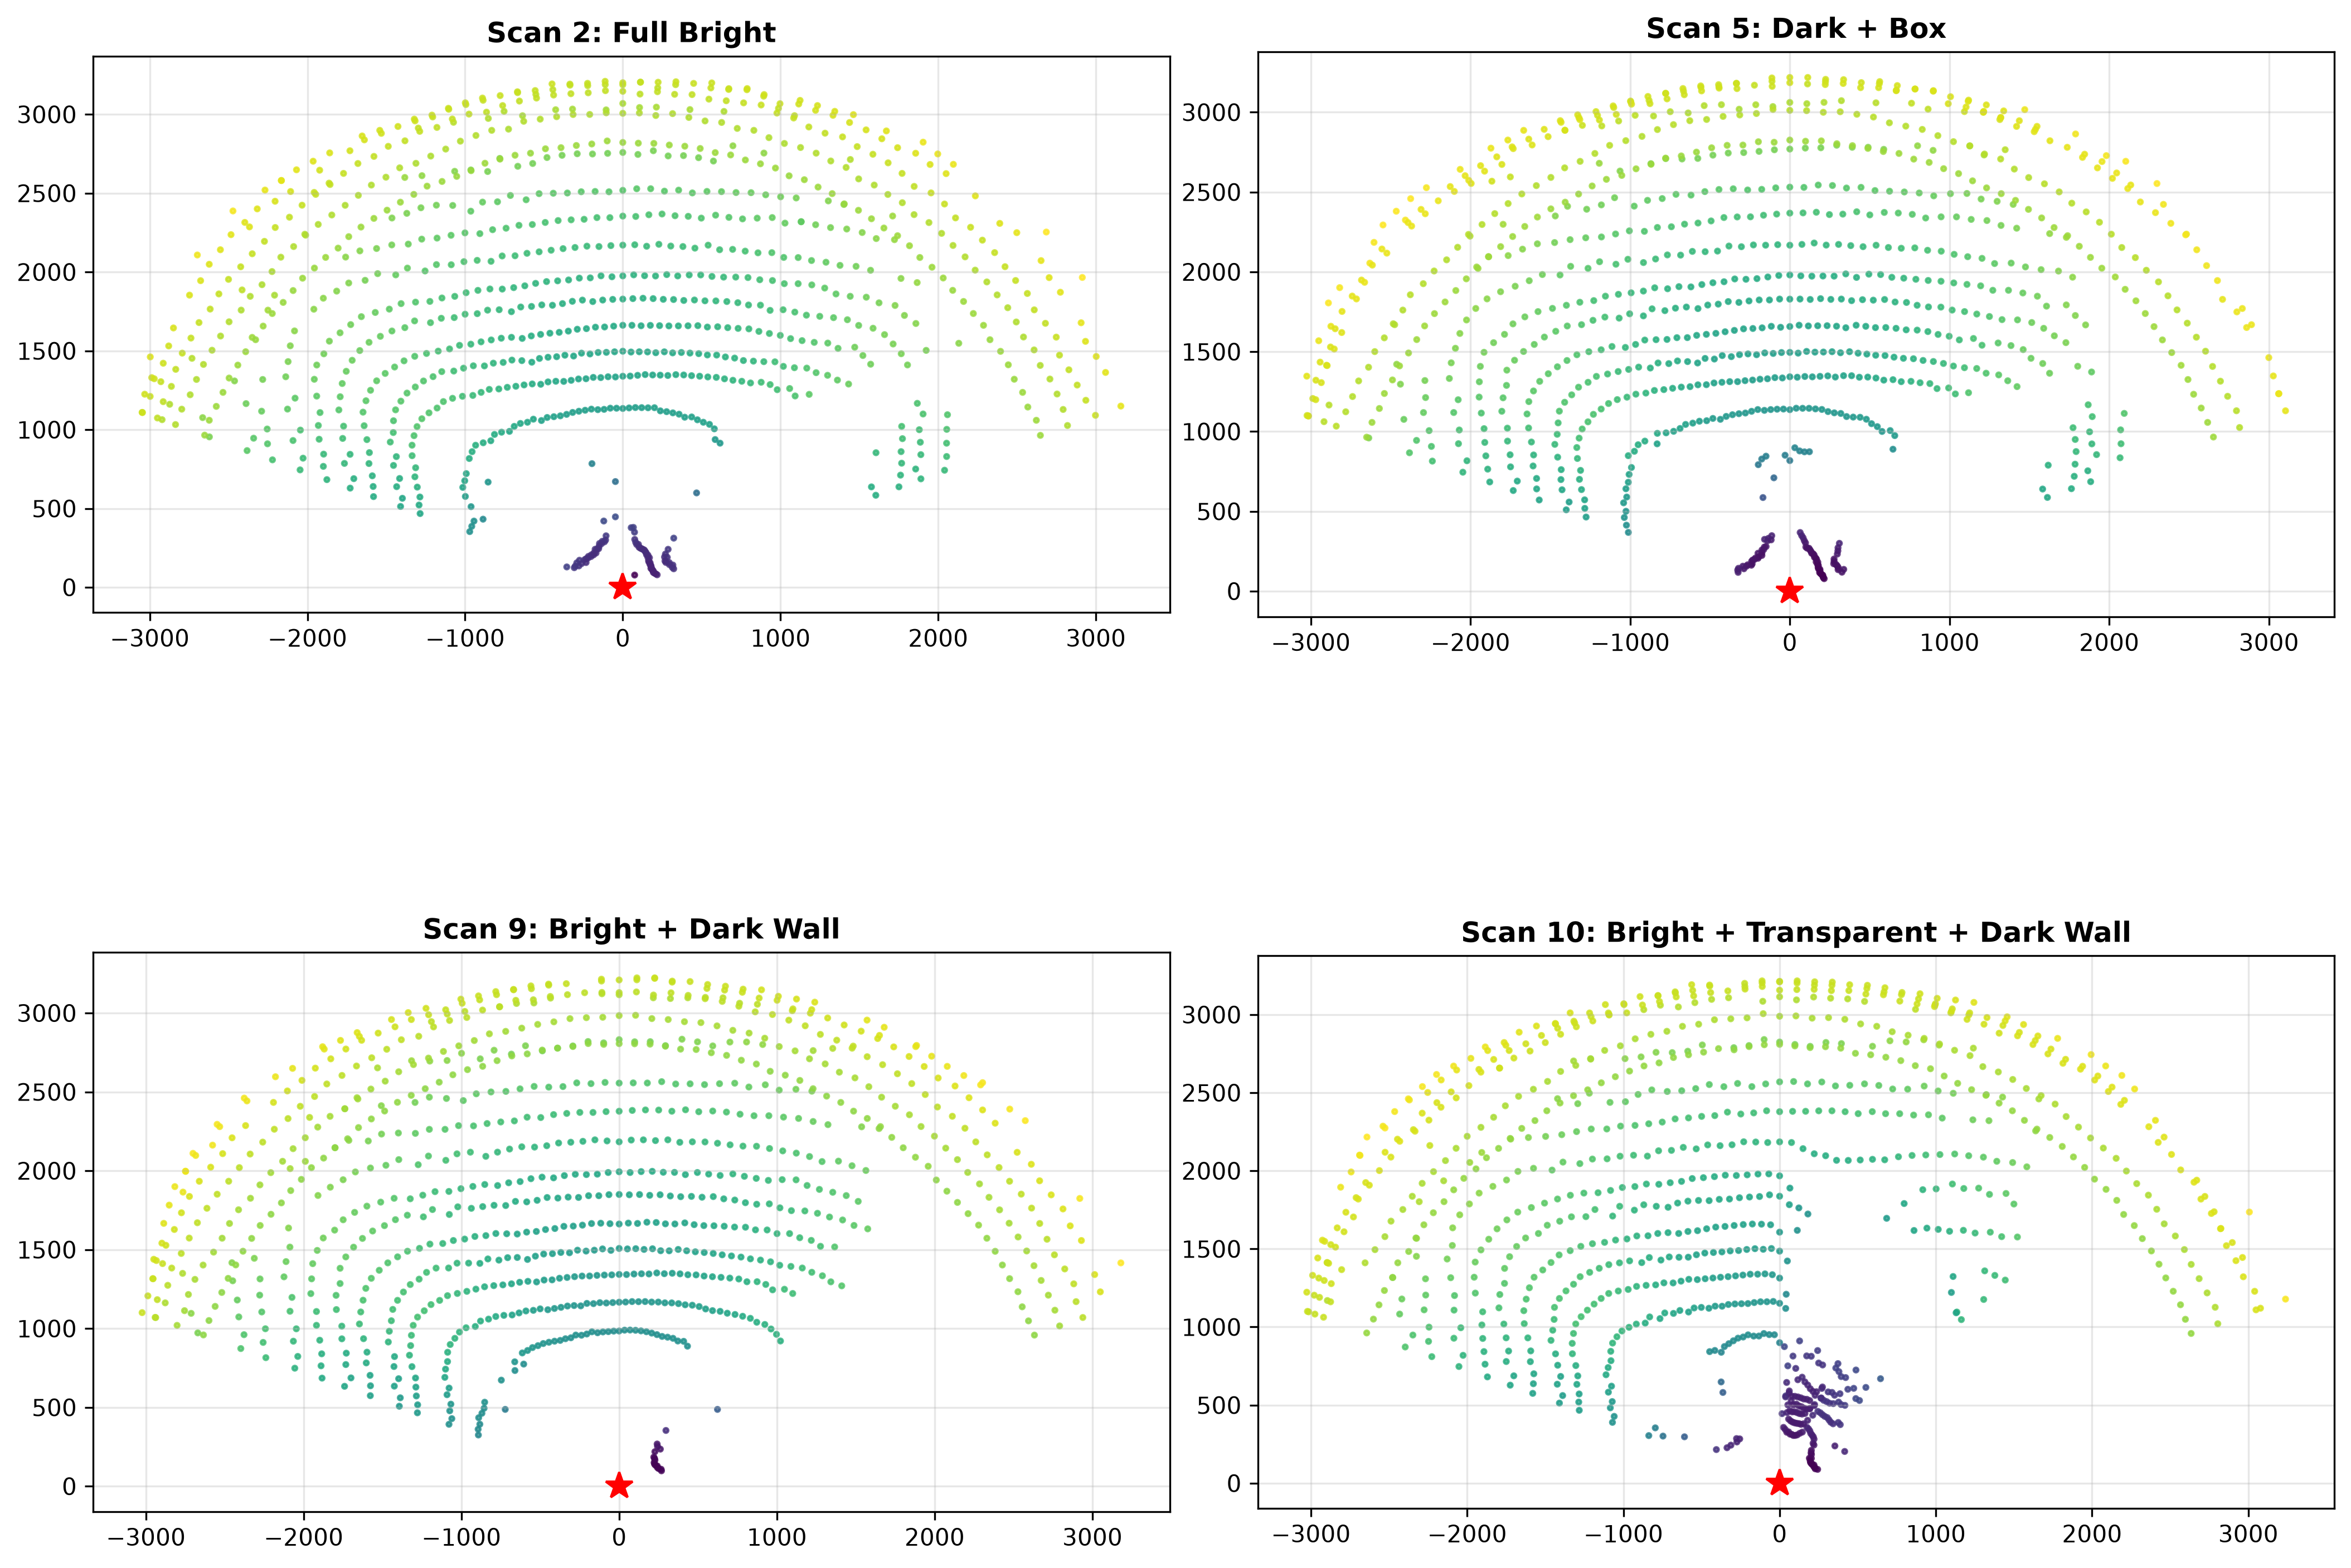
\includegraphics[width=0.95\textwidth]{figures/all_scans_mosaic.png}}
\caption{Point cloud representations of four representative test scenarios from Day 2. The ML model reduces errors across challenging cases like translucent objects and varying LED illumination.}
\label{fig:mosaic}
\end{figure*}

\subsection{Cross-Environment Transfer}
In Environment A, the uncalibrated sensor produced an MAE of 18.24 mm; in Environment B, the raw MAE increased to 934.97 mm. When XGBoost was trained on A and tested on B, MAE was 947.15 mm. The reverse produced 1049.09 mm, showing that single-environment calibration fails under domain shift.

\begin{table}[htbp]
\caption{Cross-Environment Evaluation (Mean Absolute Error)}
\begin{center}
\renewcommand{\arraystretch}{1.3}
\resizebox{\columnwidth}{!}{
\begin{tabular}{llcc}
\toprule
\textbf{Training Env.} & \textbf{Testing Env.} & \textbf{Raw MAE} & \textbf{XGBoost MAE} \\
\midrule
Day 1 (Controlled A) & Day 2 (Diverse B) & 934.97 mm & 947.15 mm \\
Day 2 (Diverse B) & Day 1 (Controlled A) & 18.24 mm & 1049.09 mm \\
\textbf{Combined A+B} & \textbf{Combined A+B} & \textbf{149.84 mm} & \textbf{22.41 mm} \\
\bottomrule
\end{tabular}
}
\label{tab:cross_eval}
\end{center}
\end{table}

\subsection{Multi-Environment Pooled Calibration}
Pooling data from both environments improved performance substantially. Raw pooled MAE was 149.84 mm, whereas XGBoost reduced the error to 22.41 mm. Because Environment A represents approximately 85\% of the dataset, this combined metric is heavily weighted toward the controlled environment; future work will evaluate per-environment metrics after pooled training.

\begin{figure}[htbp]
\centerline{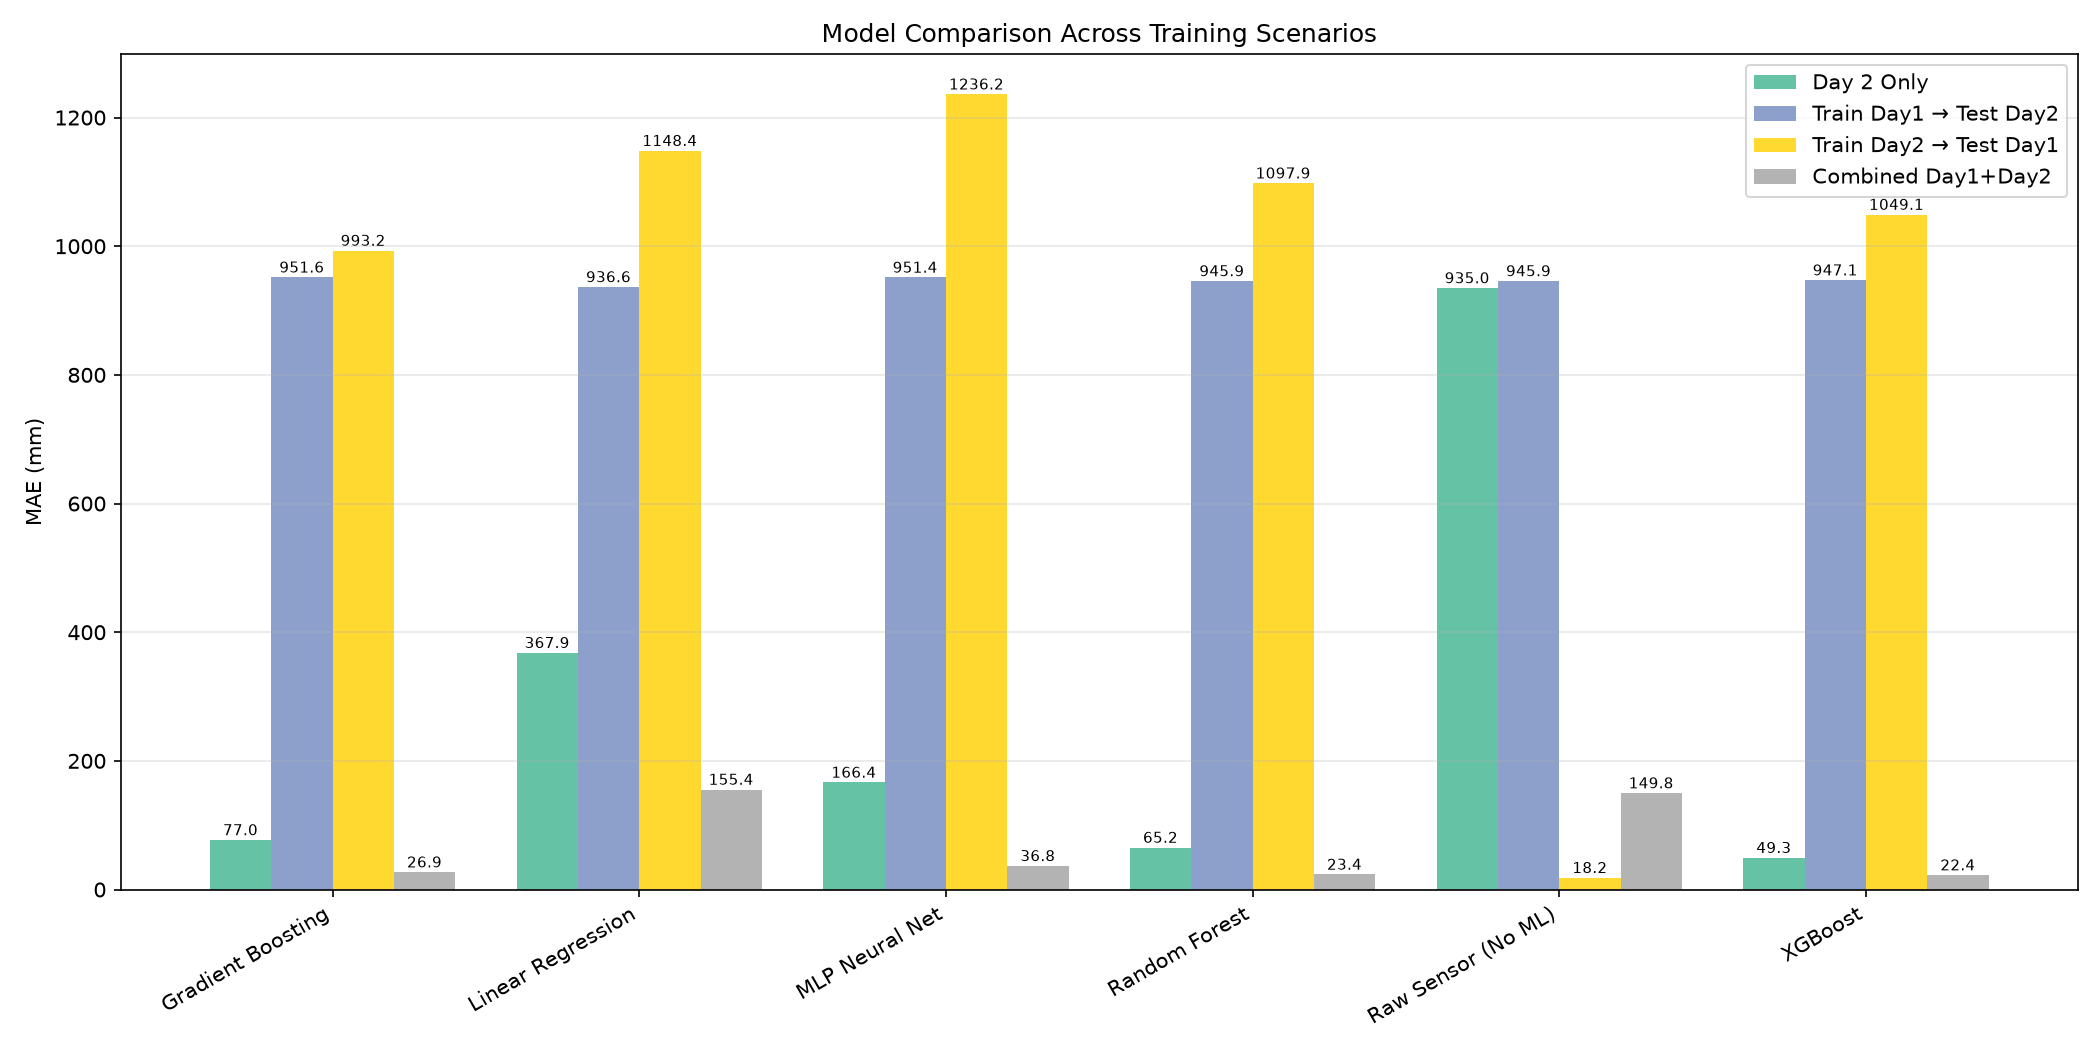
\includegraphics[width=\columnwidth]{figures/model_comparison.png}}
\caption{Model performance comparison on the Combined Dataset. Tree-based models (RF, XGBoost, DT) significantly outperform the raw sensor and linear regression.}
\label{fig:model_comp}
\end{figure}

This indicates that a single nonlinear model can represent different error regimes when exposed to heterogeneous training data. However, because the experiment uses only two environments, the result should be interpreted as pooled performance rather than unseen-domain generalization.

\begin{figure}[htbp]
\centerline{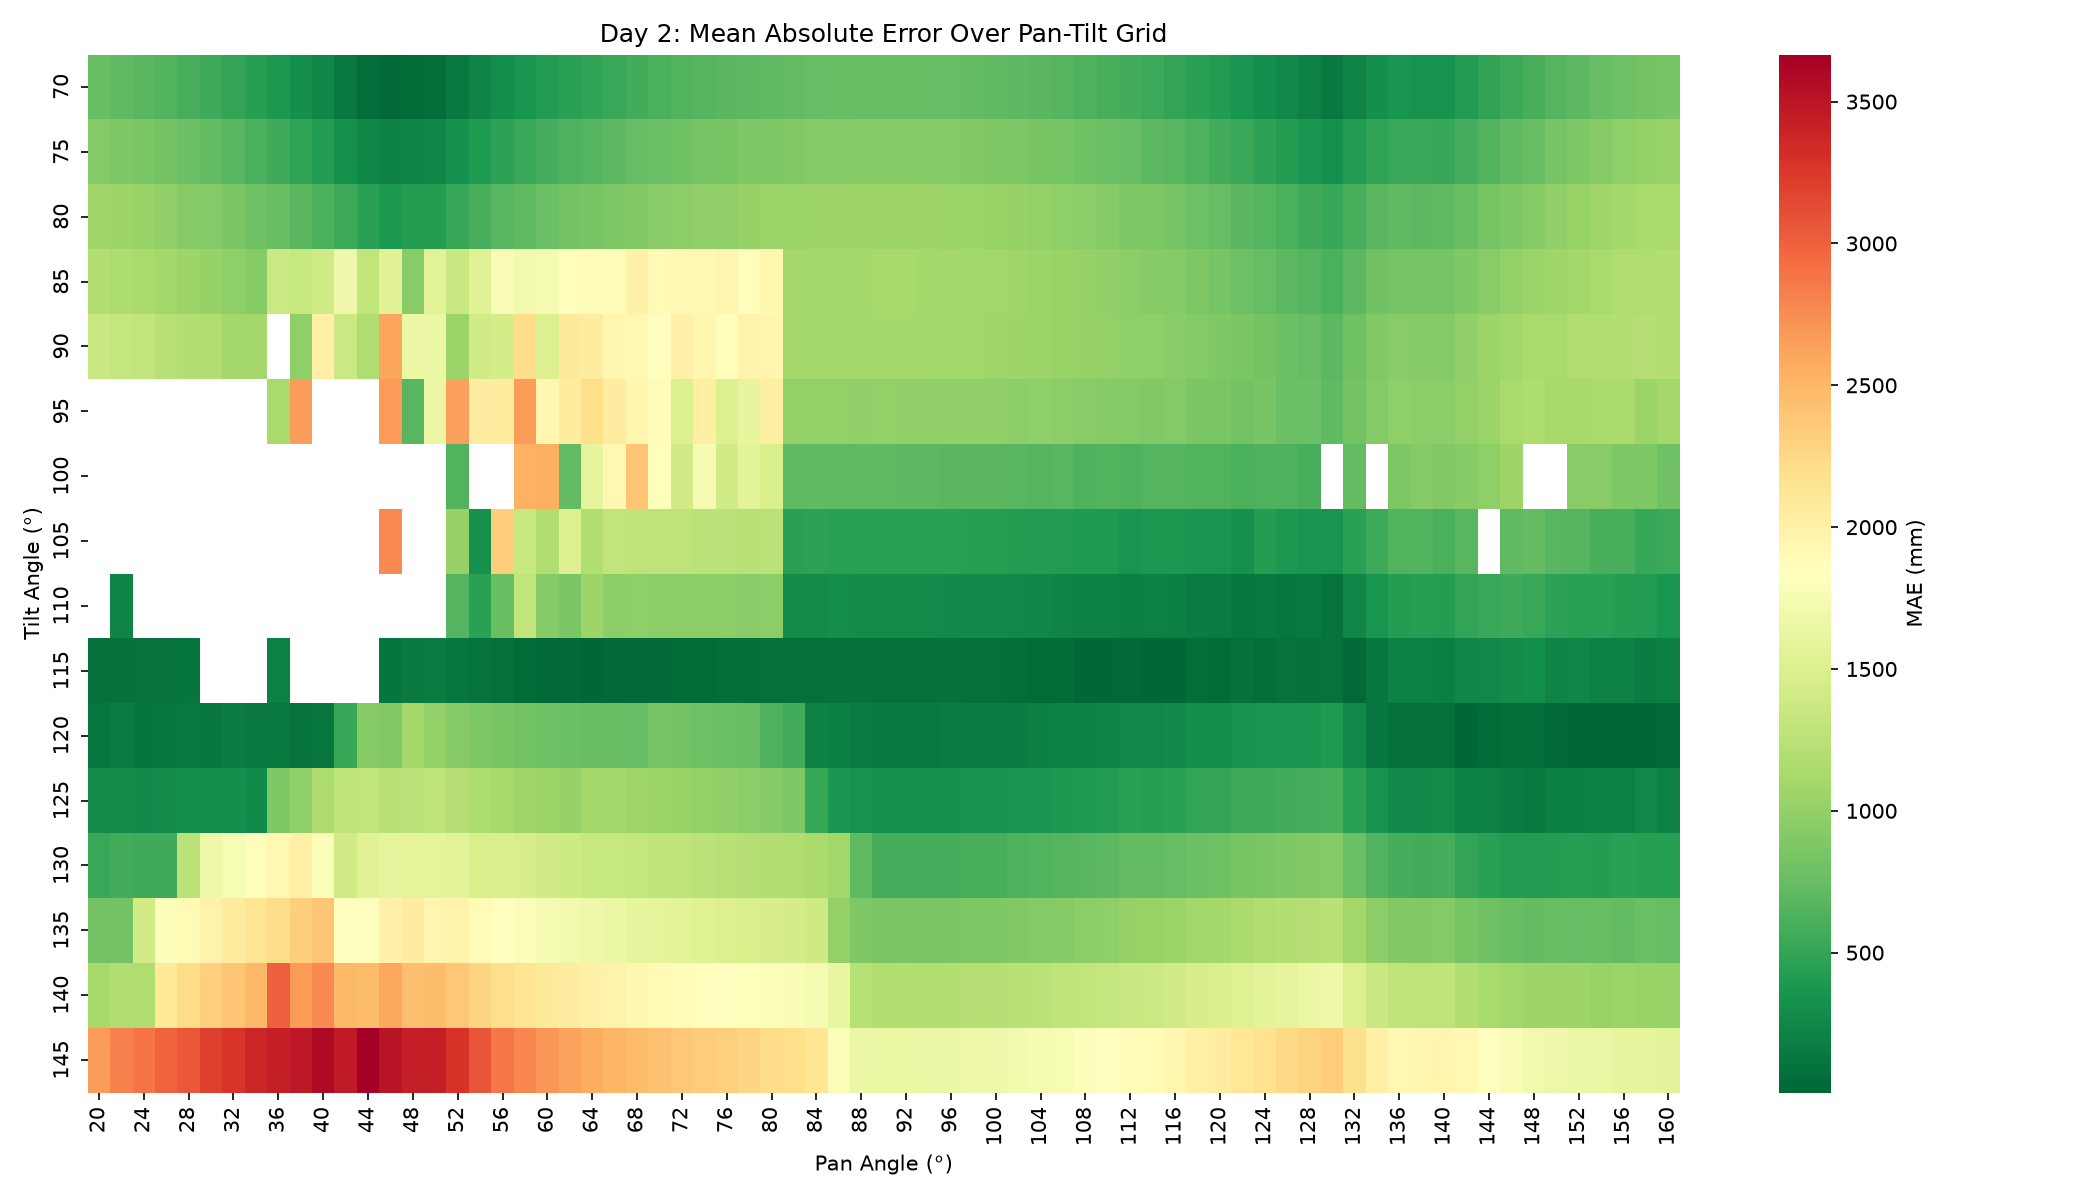
\includegraphics[width=\columnwidth]{figures/day2_error_heatmap.png}}
\caption{Heatmap of raw residual Error (uncalibrated) across the pan-tilt scanning grid in Environment B. The ML model learns to dynamically correct these high-error regions caused by specific geometric angles and lighting.}
\label{fig:heatmap}
\end{figure}



\subsection{Feature Ablation and Telemetry Limitations}
A logging failure corrupted the Day 1 signal-rate field (constant 15.0 kcps); sigma was unavailable for Day 2 and excluded. An ablation using only geometry features increased XGBoost MAE from 22.41 to 27.58 mm (Table~\ref{tab:ablation}).

\begin{table}[htbp]
\centering
\caption{Feature Ablation Study (Combined Dataset)}
\label{tab:ablation}
\begin{tabular}{@{}lc@{}}
\toprule
\textbf{Feature Set (XGBoost)} & \textbf{Test MAE (mm)} \\ \midrule
All Features (Distance, Pan, Tilt, Signal, Ambient, Temp) & 22.41 \\
Geometry Only (Distance, Pan, Tilt) & 27.58 \\
\bottomrule
\end{tabular}
\end{table}

\begin{figure}[htbp]
\centerline{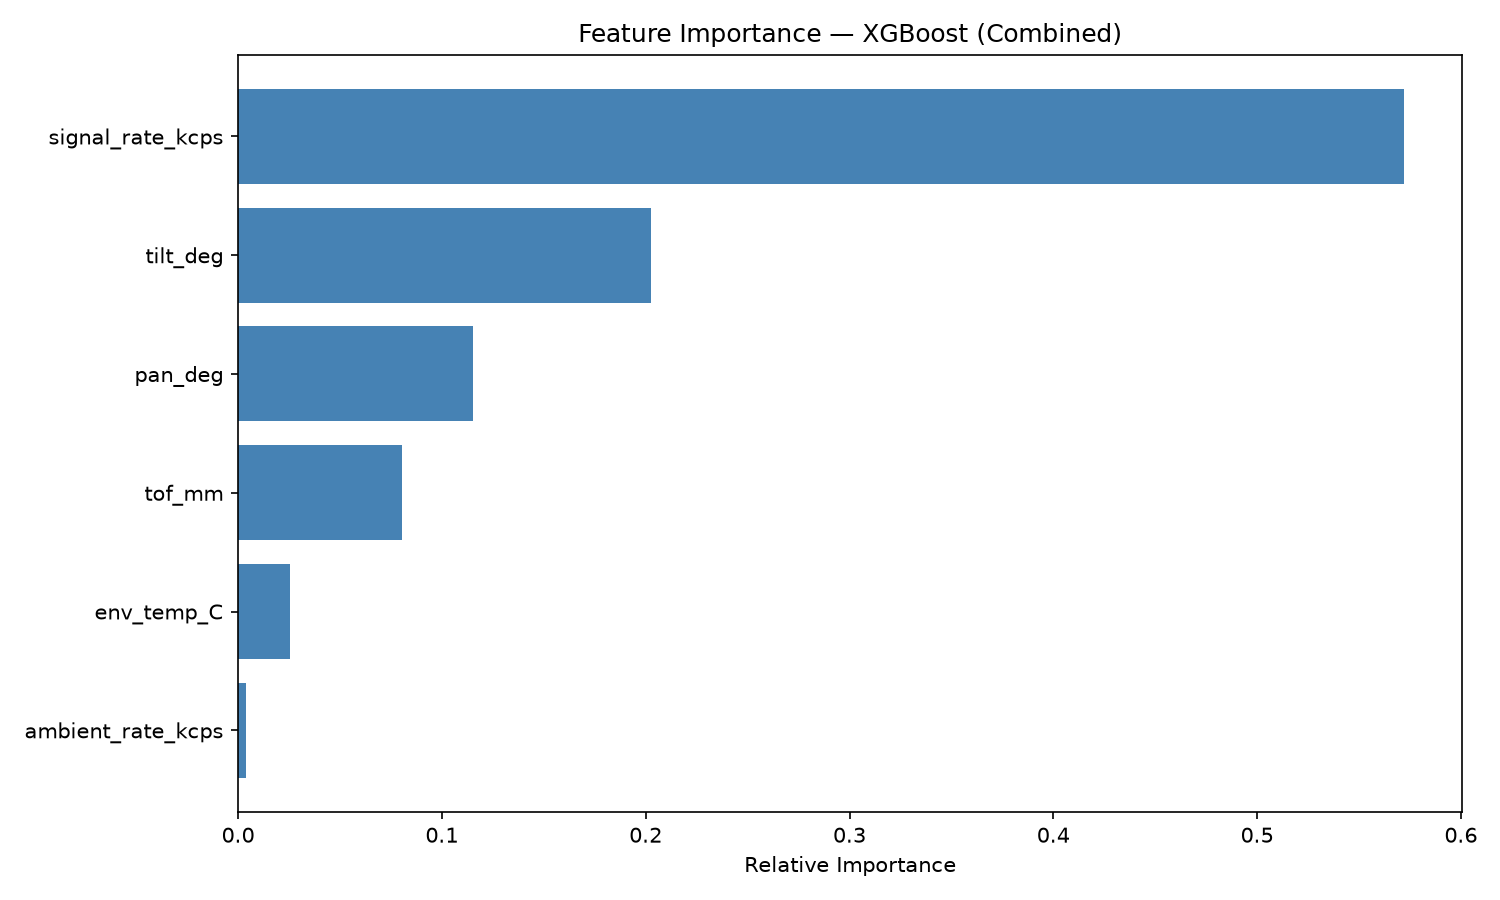
\includegraphics[width=\columnwidth]{figures/combined_feature_importance_xgboost.png}}
\caption{XGBoost Feature Importance (Combined Dataset). While raw distance is critical, signal telemetry enables the model to dynamically adjust to different environments.}
\label{fig:feat_imp}
\end{figure}



The full feature set's improvement suggests non-geometric variables contribute useful information. However, due to the corrupted Day 1 signal-rate channel, we cannot causally claim signal rate alone drives this improvement. Future work should capture complete telemetry across all environments to evaluate individual feature groups.

\begin{figure}[htbp]
\centering
\resizebox{\columnwidth}{!}{
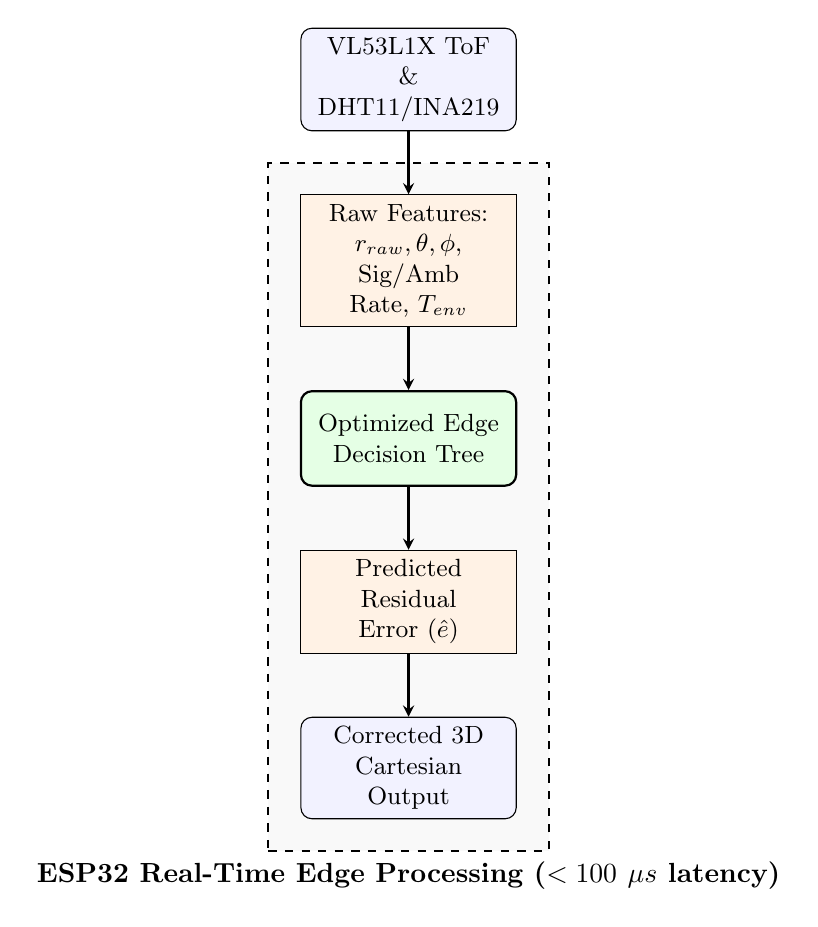
\begin{tikzpicture}[
    node distance=0.8cm,
    block/.style={rectangle, draw, fill=blue!5, text width=2.5cm, text centered, rounded corners, minimum height=1.2cm, font=\small},
    data/.style={rectangle, draw, fill=orange!10, text width=2.5cm, text centered, minimum height=1.2cm, font=\small},
    model/.style={rectangle, draw, fill=green!10, text width=2.5cm, text centered, rounded corners, minimum height=1.2cm, font=\small, thick},
    arrow/.style={thick,->,>=stealth}
]

% Nodes
\node [block] (sensor) {VL53L1X ToF \\ \& DHT11/INA219};
\node [data, below=of sensor] (raw_data) {Raw Features: \\ $r_{raw}, \theta, \phi$, \\ Sig/Amb Rate, $T_{env}$};
\node [model, below=of raw_data] (dt) {Optimized Edge \\ Decision Tree};
\node [data, below=of dt] (residual) {Predicted \\ Residual Error ($\hat{e}$)};
\node [block, below=of residual] (calibrated) {Corrected 3D \\ Cartesian Output};

% Arrows
\draw [arrow] (sensor) -- (raw_data);
\draw [arrow] (raw_data) -- (dt);
\draw [arrow] (dt) -- (residual);
\draw [arrow] (residual) -- (calibrated);

% Grouping box for ESP32
\begin{scope}[on background layer]
    \node[draw, dashed, thick, fill=gray!5, fit=(raw_data) (dt) (residual) (calibrated), inner sep=0.4cm, label=below:{\textbf{ESP32 Real-Time Edge Processing ($<100~\mu s$ latency)}}] (esp_box) {};
\end{scope}

\end{tikzpicture}
}
\vspace{0.1cm}
\caption{System architecture and on-device data flow for real-time residual calibration.}
\label{fig:architecture}
\end{figure}

\subsection{TinyML Model Selection and ESP32 Deployment}
XGBoost achieved the best accuracy but generated $\sim$40 MB of source code. The generated source-code size increased substantially with tree depth, motivating the selection of depth 12 as a practical code-size/accuracy compromise.

\begin{table}[htbp]
\centering
\caption{Edge Deployment Characteristics (ESP32)}
\label{tab:deployment}
\resizebox{\columnwidth}{!}{
\begin{tabular}{@{}llcc@{}}
\toprule
\textbf{Model Architecture} & \textbf{Test MAE} & \textbf{Generated Code Size} & \textbf{Latency} \\ \midrule
Decision Tree (Depth 10) & 26.52 mm & 160.2 KB & $<100~\mu$s \\
\textbf{Decision Tree (Depth 12)} & \textbf{23.42 mm} & \textbf{453.8 KB} & \textbf{$<100~\mu$s} \\
Decision Tree (Depth 15) & 21.92 mm & 1,212.7 KB & Impractical size \\
\bottomrule
\end{tabular}
}
\end{table}

The depth-12 tree provided the optimal accuracy-memory trade-off, achieving 23.42 mm test MAE with 453.8 KB of generated C source code. The transpiled model compiled directly onto the ESP32. Inference latency was measured over 10,000 consecutive executions using the ESP32 \texttt{micros()} timer (excluding I2C and serial overhead), averaging under 100 $\mu$s---negligible relative to the sensor's 50 ms budget.

\subsection{Point-Cloud Reconstruction}
Calibrated ranges were converted to Cartesian coordinates. In the controlled environment, calibration produced flatter planar surfaces (Fig.~\ref{fig:day1_cloud}). In Environment B, large distortions and multipath artifacts around obstacles were substantially reduced after calibration (Fig.~\ref{fig:mosaic}).

\begin{figure}[htbp]
\centering
\begin{minipage}{0.45\columnwidth}
  \centering
  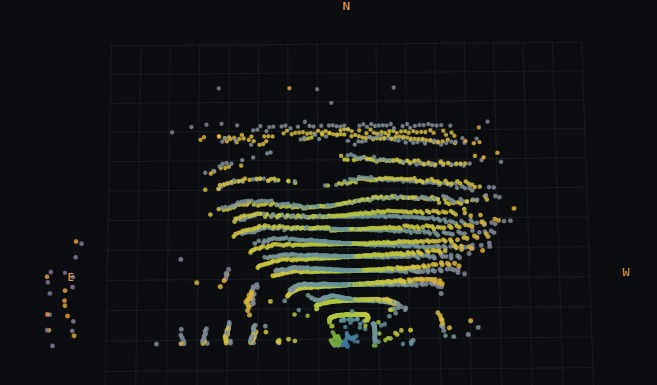
\includegraphics[width=\linewidth]{figures/Cloud point Mapping.png}
  \centerline{(a) Upper view}
\end{minipage}\hfill
\begin{minipage}{0.45\columnwidth}
  \centering
  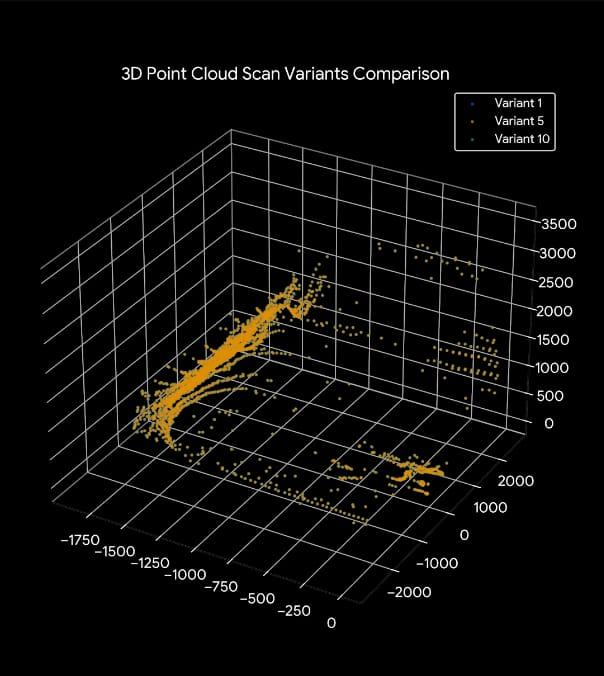
\includegraphics[width=\linewidth]{figures/3D Cloud point Mapping-1.png}
  \centerline{(b) Side view}
\end{minipage}
\caption{Day 1 3D point cloud reconstruction from multiple perspectives.}
\label{fig:day1_cloud}
\end{figure}

\section{Discussion}

\subsection{Cross-Environment Transfer}
The cross-environment experiments show that calibration learned in one room can become invalid under different conditions. Sensor error depends not only on distance but also on lighting, reflectivity, multipath geometry, and scan configuration. Pooled training across multiple error regimes substantially improves aggregate performance, though this should not be interpreted as proof of unseen-domain generalization.

\subsection{Embedded Accuracy-Memory Trade-off}
The highest-accuracy model (XGBoost) was impractical for deployment. A depth-12 decision tree increased MAE only slightly while reducing the footprint enough for embedded use, avoiding dependence on external compute.

\subsection{Limitations}
This study has four limitations: only two environments were tested; the Day 1 signal-rate was corrupted; manual ground-truth introduces label uncertainty; and the 80/20 point-level split risks spatial data leakage, meaning the 22.41 mm MAE is likely an optimistic bound. Future work must use scan-level holdout protocols, capture complete telemetry, and test on a third unseen environment.

\section{Conclusion}
This paper presented a low-cost pan-tilt ToF mapping platform and evaluated ML-based residual calibration across two distinct indoor environments. Environment-specific models transferred poorly, with cross-environment MAEs near one meter. Pooled training reduced aggregate MAE from 149.84 mm to 22.41 mm. A depth-12 decision tree achieved 23.42 mm MAE, requiring 453.8 KB of C source code and executing in under 100 $\mu$s on an ESP32.

The results support two conclusions: calibration for low-cost ToF mapping should be trained on heterogeneous conditions, and compact tree models can provide nearly the same accuracy as larger ensembles while remaining deployable on resource-constrained microcontrollers. Future work will focus on blind evaluation in additional environments, improved ground-truth metrology, and complete telemetry capture.

\bibliographystyle{IEEEtran}
\bibliography{references}

\end{document}
